\documentclass{article} % For LaTeX2e
\usepackage{etex}
\usepackage[T1]{fontenc}
\usepackage[bitstream-charter]{mathdesign}
\usepackage[scaled=0.92]{PTSans}
\renewcommand*\ttdefault{lmvtt}
\usepackage{exscale}

\usepackage[final,expansion=alltext]{microtype}
\usepackage[english]{babel}
\usepackage{ragged2e}

\usepackage{amsmath}
\usepackage{graphicx}                               % graphics
\usepackage{booktabs, array}                        % nice tables
\usepackage[algoruled]{algorithm2e}                 % pseudocode
\usepackage[numbers,sort]{natbib}                   % better bibliography
\usepackage{cleveref}                               % the best package ever
\usepackage[acronym,smallcaps,nowarn]{glossaries}   % second best package ever

% COLORS
\newcommand{\gray}[1]{\textcolor{black!60}{#1}}
\newcommand{\blu}[1]{\textcolor{jblue}{#1}}

\usepackage{iclr2017_conference}
\newacronym{ELBO}{elbo}{evidence lower bound}
\newacronym{KL}{kl}{Kullback-Leibler}

\newacronym{DEF}{def}{deep exponential family}
\newacronym{DLGM}{dlgm}{deep latent Gaussian model}
\newacronym{DRAW}{draw}{Deep Recurrent Attentive Writer}

\newacronym{MF}{mf}{mean-field}
\newacronym{VGP}{vgp}{variational Gaussian process}
\newacronym{BBVI}{bbvi}{black box variational inference}
\newacronym{ADVI}{advi}{automatic differentiation variational inference}
\newacronym{NF}{nf}{normalizing flows}
\newacronym{CVI}{cvi}{copula variational inference}
\newacronym{VAE}{vae}{variational autoencoder}
\newacronym{IWAE}{iwae}{importance weighted autoencoder}
\newacronym{NVIL}{nvil}{neural variational inference}
\newacronym{MIXTURE}{mixture}{}
\newacronym{DSVI}{dsvi}{}

\newacronym{VI}{vi}{variational inference}
\newacronym{EP}{ep}{expectation propagation}

\newacronym{LS}{ls}{Langevin-Stein}
\newacronym{OPVI}{opvi}{operator variational inference}

\DeclareRobustCommand{\mb}[1]{\ensuremath{\boldsymbol{\mathbf{#1}}}}
\DeclareRobustCommand{\mbf}[1]{\ensuremath{\textbf{#1}}}
\DeclareMathOperator*{\argmax}{arg\,max}
\DeclareMathOperator*{\argmin}{arg\,min}


\newcommand{\KL}[2]{\ensuremath{\textrm{KL}\left(#1\;\|\;#2\right)}}

\renewcommand{\mid}{~\vert~}

\newcommand{\mbw}{\mb{w}}
\newcommand{\mbW}{\mb{W}}

\newcommand{\mbx}{\mb{x}}
\newcommand{\mbX}{\mbf{X}}

\newcommand{\mby}{\mb{y}}
\newcommand{\mbY}{\mbf{Y}}

\newcommand{\mbz}{\mb{z}}
\newcommand{\mbZ}{\mb{Z}}

\newcommand{\mbI}{\mbf{I}}
\newcommand{\mbone}{\mbf{1}}

\newcommand{\mbL}{\mbf{L}}

\newcommand{\mbtheta}{\mb{\theta}}
\newcommand{\mbTheta}{\mb{\Theta}}
\newcommand{\mbomega}{\mb{\omega}}
\newcommand{\mbOmega}{\mb{\Omega}}
\newcommand{\mbsigma}{\mb{\sigma}}
\newcommand{\mbSigma}{\mb{\Sigma}}
\newcommand{\mbphi}{\mb{\phi}}
\newcommand{\mbPhi}{\boldsymbol{\Phi}}
% \newcommand{\mblambda}{\mb{\lambda}}

\newcommand{\mbalpha}{\mb{\alpha}}
\newcommand{\mbbeta}{\mb{\beta}}
\newcommand{\mbgamma}{\mb{\gamma}}
\newcommand{\mbeta}{\mb{\eta}}
\newcommand{\mbmu}{\mb{\mu}}
\newcommand{\mbrho}{\mb{\rho}}
\newcommand{\mblambda}{\mb{\lambda}}
\newcommand{\mbzeta}{\mb{\zeta}}

\newcommand\dif{\mathop{}\!\mathrm{d}}
\newcommand{\diag}{\textrm{diag}}
\newcommand{\supp}{\textrm{supp}}

\newcommand{\E}{\mathbb{E}}
\newcommand{\bbH}{\mathbb{H}}
\newcommand{\Var}{\mathbb{V}\textrm{ar}}

\newcommand{\bbN}{\mathbb{N}}
\newcommand{\bbZ}{\mathbb{Z}}
\newcommand{\bbR}{\mathbb{R}}
\newcommand{\bbS}{\mathbb{S}}

\newcommand{\cL}{\mathcal{L}}

\newcommand{\cN}{\mathcal{N}}
\newcommand{\cT}{\mathcal{T}}
\newcommand{\Gam}{\textrm{Gam}}
\newcommand{\InvGam}{\textrm{InvGam}}

\usepackage{tikz}
\usetikzlibrary{bayesnet}

\pgfdeclarelayer{edgelayer}
\pgfdeclarelayer{nodelayer}
\pgfsetlayers{edgelayer,nodelayer,main}

\definecolor{hexcolor0xbfbfbf}{rgb}{0.749,0.749,0.749}

\tikzset{>=latex}
\tikzstyle{none}   = [inner sep=0pt]
\tikzstyle{line}   = [-,
                      thick,
                      shorten <=1pt,
                      shorten >=1pt]
\tikzstyle{arrow}  = [->,
                      thick,
                      shorten <=1pt,
                      shorten >=1pt]
\tikzstyle{ardash} = [dashed,
                      ->,
                      thick,
                      shorten <=1pt,
                      shorten >=1pt]

\tikzstyle{empty}=[
                   circle,
                   opacity=0.0,
                   text opacity=1.0,
                   inner sep=0pt
                  ]

\tikzstyle{box}=[
                 rectangle,
                 fill=White,
                 thick,
                 draw=Black,
                 inner sep=7pt
                ]

\tikzstyle{filled}=[
                    circle,
                    thick,
                    fill=hexcolor0xbfbfbf,
                    draw=Black
                   ]

\tikzstyle{hollow}=[
                    circle,
                    thick,
                    fill=White,
                    draw=Black
                   ]

\tikzstyle{param}=[
                   rectangle,
                   fill=Black,
                   draw=Black,
                   inner sep=0pt,
                   minimum width=4pt,
                   minimum height=4pt
                  ]

\tikzstyle{paramhollow}=[
                         rectangle,
                         thick,
                         fill=White,
                         draw=Black,
                         inner sep=0pt,
                         minimum
                         width=4pt,
                         minimum height=4pt
                        ]

\usepackage{pgfplots}                               % PGFPLOTS baby!
\pgfplotsset{compat=newest}
\pgfplotsset{plot coordinates/math parser=false}
% \usepgfplotslibrary{statistics}


\title{}
\author{}

\newcommand{\fix}{\marginpar{FIX}}
\newcommand{\new}{\marginpar{NEW}}

\iclrfinalcopy

\begin{document}

\maketitle

\begin{figure}[t]
\centering
\begin{lstlisting}[language=python]
# univariate normal
Normal(loc=0.0, scale=1.0)
# vector of 5 univariate normals
Normal(loc=tf.zeros(5), scale=tf.ones(5))
# 2 x 3 matrix of Exponentials
Exponential(rate=tf.ones([2, 3]))
\end{lstlisting}
\caption{}
\end{figure}

\begin{figure}[t]
\begin{subfigure}{0.3\columnwidth}
  \centering
\begin{lstlisting}[language=python]
theta = Beta(1.0, 1.0)
x = Bernoulli(probs=tf.ones(50) * theta)
\end{lstlisting}
\end{subfigure}%
\begin{subfigure}{0.65\columnwidth}
  \centering
  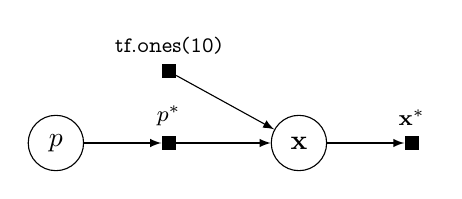
\begin{tikzpicture}[x=1.7cm,y=1.8cm,scale=0.9]
%\begin{tikzpicture}[scale=0.6]

  % Nodes
  \node[latent] (p) {$p$};
  \factor[right=of p, xshift=0.3cm] {thetastar} {$p^*$} {} {};

  \factor[above=of thetastar] {n} {\texttt{tf.ones(10)}} {} {};
  \node[latent, right=of thetastar, xshift=-0.5cm] (x) {$\mbx$};
  \factor[right=of x, xshift=0.3cm] {xstar} {$\mbx^*$} {} {};

  % Edges
  \edge{p}{thetastar};
  \edge{thetastar}{x};
  \edge{n}{x};
  \edge{x}{xstar};

\end{tikzpicture}

\end{subfigure}
\caption{}
\end{figure}

\begin{figure}[t]
\begin{subfigure}{1.0\columnwidth}
  \centering
\begin{lstlisting}[language=python]
X = tf.placeholder(tf.float32, [N, D])
f = MultivariateNormalTriL(loc=tf.zeros(N),
                           scale_tril=tf.cholesky(rbf(X)))
y = Bernoulli(logits=f)
\end{lstlisting}
\end{subfigure}%
% \begin{subfigure}{1.0\columnwidth}
%   \centering
%   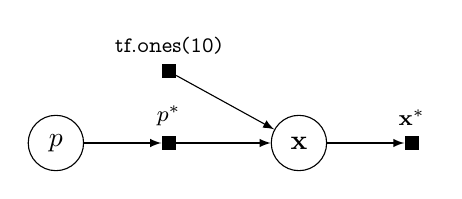
\begin{tikzpicture}[x=1.7cm,y=1.8cm,scale=0.9]
%\begin{tikzpicture}[scale=0.6]

  % Nodes
  \node[latent] (p) {$p$};
  \factor[right=of p, xshift=0.3cm] {thetastar} {$p^*$} {} {};

  \factor[above=of thetastar] {n} {\texttt{tf.ones(10)}} {} {};
  \node[latent, right=of thetastar, xshift=-0.5cm] (x) {$\mbx$};
  \factor[right=of x, xshift=0.3cm] {xstar} {$\mbx^*$} {} {};

  % Edges
  \edge{p}{thetastar};
  \edge{thetastar}{x};
  \edge{n}{x};
  \edge{x}{xstar};

\end{tikzpicture}

% \end{subfigure}
\caption{}
\end{figure}

\begin{figure}[t]
\begin{subfigure}{1.0\columnwidth}
  \centering
\begin{lstlisting}[language=python]
X = Normal(loc=tf.zeros([N, Q]), scale=tf.ones([N, Q]))
f = MultivariateNormalTriL(loc=tf.zeros([N, D]),
                           scale_tril=tf.cholesky(rbf(X)))
y = Bernoulli(logits=f)
\end{lstlisting}
\end{subfigure}%
% \begin{subfigure}{1.0\columnwidth}
%   \centering
%   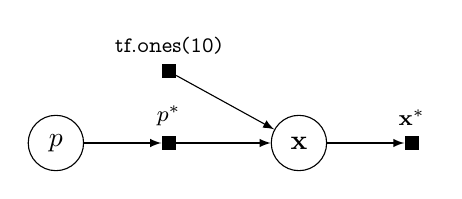
\begin{tikzpicture}[x=1.7cm,y=1.8cm,scale=0.9]
%\begin{tikzpicture}[scale=0.6]

  % Nodes
  \node[latent] (p) {$p$};
  \factor[right=of p, xshift=0.3cm] {thetastar} {$p^*$} {} {};

  \factor[above=of thetastar] {n} {\texttt{tf.ones(10)}} {} {};
  \node[latent, right=of thetastar, xshift=-0.5cm] (x) {$\mbx$};
  \factor[right=of x, xshift=0.3cm] {xstar} {$\mbx^*$} {} {};

  % Edges
  \edge{p}{thetastar};
  \edge{thetastar}{x};
  \edge{n}{x};
  \edge{x}{xstar};

\end{tikzpicture}

% \end{subfigure}
\caption{}
\end{figure}

\begin{figure}[t]
\begin{subfigure}{1.0\columnwidth}
  \centering
\begin{lstlisting}[language=python]
X = Normal(loc=tf.zeros([N, Q]), scale=tf.ones([N, Q]))
h1 = MultivariateNormalTriL(loc=tf.zeros([N, H1]),
                            scale_tril=tf.cholesky(rbf(X)))
h2 = MultivariateNormalTriL(loc=tf.zeros([N, H2]),
                            scale_tril=tf.cholesky(rbf(h1)))
f = MultivariateNormalTriL(loc=tf.zeros([N, D]),
                           scale_tril=tf.cholesky(rbf(h2)))
y = Bernoulli(logits=f)
\end{lstlisting}
\end{subfigure}%
% \begin{subfigure}{1.0\columnwidth}
%   \centering
%   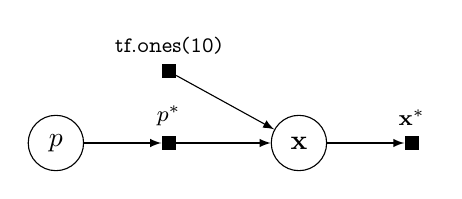
\begin{tikzpicture}[x=1.7cm,y=1.8cm,scale=0.9]
%\begin{tikzpicture}[scale=0.6]

  % Nodes
  \node[latent] (p) {$p$};
  \factor[right=of p, xshift=0.3cm] {thetastar} {$p^*$} {} {};

  \factor[above=of thetastar] {n} {\texttt{tf.ones(10)}} {} {};
  \node[latent, right=of thetastar, xshift=-0.5cm] (x) {$\mbx$};
  \factor[right=of x, xshift=0.3cm] {xstar} {$\mbx^*$} {} {};

  % Edges
  \edge{p}{thetastar};
  \edge{thetastar}{x};
  \edge{n}{x};
  \edge{x}{xstar};

\end{tikzpicture}

% \end{subfigure}
\caption{}
\end{figure}

\begin{figure}[t]
\begin{subfigure}{0.3\columnwidth}
  \centering
  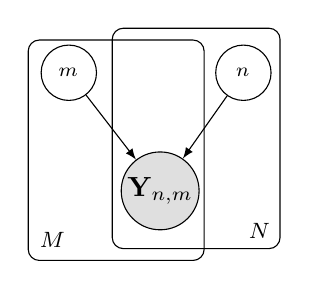
\begin{tikzpicture}

  % Nodes
  \node[latent]               (U)      {$\mbU_{m}$} ;
  \node[obs, right=0.3cm of U, yshift=-1.5cm] (Y)    {$\mbY_{n,m}$} ;
  \node[latent, right=1.5cm of U] (V)    {$\mbV_{n}$} ;

  % Edges
  \edge{U}{Y};
  \edge{V}{Y};

  % Plates
  \plate[inner sep=0.1cm,yshift=-0.05cm,xshift=-0.05cm,
    label={[xshift=17pt,yshift=14pt]south west:$M$}] {plate1} {
    (U)(Y)
  } {};
  \plate[inner sep=0.1cm,yshift=0.1cm,
    label={[xshift=-15pt,yshift=13pt]south east:$N$}] {plate2} {
    (V)(Y)
  } {};

\end{tikzpicture}

\end{subfigure}%
\begin{subfigure}{0.7\columnwidth}
\begin{lstlisting}[language=python]
N = 10
M = 10
K = 5  # latent dimension

U = Normal(loc=tf.zeros([M, K]), sigma=tf.ones([M, K]))
V = Normal(loc=tf.zeros([N, K]), sigma=tf.ones([N, K]))
Y = Normal(loc=tf.matmul(U, V, transpose_b=True), sigma=tf.ones([N, M]))
\end{lstlisting}
\end{subfigure}
\caption{}
\end{figure}

\begin{figure}[t]
\begin{subfigure}{0.225\columnwidth}
  \centering
  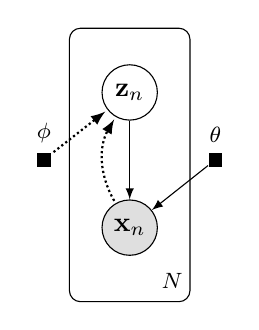
\begin{tikzpicture}

  % Nodes
  \node[latent] (z) {$\mbz_n$};
  \node[obs, below=of z] (x) {$\mbx_n$};

  \factor[empty, below=of z] {h} {} {} {};
  \factor[right=of h, xshift=0.5cm] {theta} {$\theta$} {} {};
  \factor[left=of h, xshift=-0.5cm] {phi} {$\phi$} {} {};

  % Edges
  \edge{z}{x};
  \draw[style=arrow, densely dotted, bend left] (x) to (z);
  \edge{theta}{x};
  \draw[style=arrow, densely dotted] (phi) to (z);

  % Plates
  \plate[inner sep=0.4cm, yshift=0.05cm,
    label={[xshift=-14pt,yshift=14pt]south east:$N$}] {plate1} {
    (z)(x)
  } {};

\end{tikzpicture}

\end{subfigure}%
\begin{subfigure}{0.65\columnwidth}
  \centering
\begin{lstlisting}[language=python]
# Probabilistic model
z = Normal(loc=tf.zeros([N, d]), scale=tf.ones([N, d]))
h = Dense(256, activation='relu')(z)
x = Bernoulli(logits=Dense(28 * 28, activation=None)(h))

# Variational model
qx = tf.placeholder(tf.float32, [N, 28 * 28])
qh = Dense(256, activation='relu')(qx)
qz = Normal(loc=Dense(d, activation=None)(qh),
            scale=Dense(d, activation='softplus')(qh))
\end{lstlisting}
\end{subfigure}
\caption{}
\end{figure}

\begin{figure}[t]
\centering
\begin{lstlisting}[language=python]
N = 1000  # number of data points
d = 10  # latent dimensionality

# DATA
x_data = np.loadtxt('mnist.txt', np.float32)

# MODEL
z = Normal(loc=tf.zeros([N, d]), scale=tf.ones([N, d]))
h = Dense(256, activation='relu')(z)
x = Bernoulli(logits=Dense(28 * 28, activation=None)(h))

# INFERENCE
qx = tf.placeholder(tf.float32, [N, 28 * 28])
qh = Dense(256, activation='relu')(qx)
qz = Normal(loc=Dense(d, activation=None)(qh),
            scale=Dense(d, activation='softplus')(qh))

inference = ed.KLqp({z: qz}, data={x: x_data, qx: x_data})
inference.run()
\end{lstlisting}

\begin{lstlisting}[language=python]
N = 1000  # number of data points
d = 10  # latent dimensionality

# DATA
x_data = np.loadtxt('mnist.txt', np.float32)

# MODEL
z = Normal(loc=tf.zeros([N, d]), scale=tf.ones([N, d]))
h = Dense(256, activation='relu')(z)
x = Bernoulli(logits=Dense(28 * 28, activation=None)(h))

# INFERENCE
T = 10000  # number of samples
qz = Empirical(params=tf.Variable(tf.zeros([T, N, d])))

inference = ed.HMC({z: qz}, data={x: x_data})
inference.run()
\end{lstlisting}
\caption{}
\end{figure}

\begin{figure}[t]
\begin{lstlisting}[language=python]
inference = ed.Inference({beta: qbeta, z: qz}, data={x: x_train})
\end{lstlisting}

\begin{lstlisting}[language=Python]
qbeta = Normal(loc=tf.Variable(tf.zeros([K, D])),
                scale=tf.exp(tf.Variable(tf.zeros([K, D]))))
qz = Categorical(logits=tf.Variable(tf.zeros([N, K])))

inference = ed.VariationalInference({beta: qbeta, z: qz}, data={x: x_train})
\end{lstlisting}

\begin{lstlisting}[language=Python]
T = 10000  # number of samples
qbeta = Empirical(params=tf.Variable(tf.zeros([T, K, D])))
qz = Empirical(params=tf.Variable(tf.zeros([T, N])))

inference = ed.MonteCarlo({beta: qbeta, z: qz}, data={x: x_train})
\end{lstlisting}
\caption{}
\end{figure}

\begin{figure}[t]
\centering
\begin{lstlisting}[language=python]
def generative_network(eps):
  h = Dense(256, activation='relu')(eps)
  return Dense(28 * 28, activation=None)(h)

def discriminative_network(x):
  h = Dense(28 * 28, activation='relu')(x)
  return Dense(h, activation=None)(1)

# Probabilistic model
eps = Normal(loc=tf.zeros([N, d]), scale=tf.ones([N, d]))
x = generative_network(eps)

inference = ed.GANInference(data={x: x_train},
    discriminator=discriminative_network)
inference.run()
\end{lstlisting}
\begin{lstlisting}[language=python]
def generative_network(eps):
  h = Dense(256, activation='relu')(eps)
  return Dense(28 * 28, activation=None)(h)

def discriminative_network(x):
  h = Dense(28 * 28, activation='relu')(x)
  return Dense(h, activation=None)(1)

# Probabilistic model
eps = Normal(loc=tf.zeros([N, d]), scale=tf.ones([N, d]))
x = generative_network(eps)

inference = ed.WGANInference(data={x: x_train},
    discriminator=discriminative_network)
inference.run()
\end{lstlisting}
\caption{}
\end{figure}

\begin{table}[t]
\glsunset{VAE}
\centering
\begin{tabular}{lcc}
\toprule
Inference method & Neg. log-likelihood
\\
\midrule
\gls{VAE} \gray{\small [Kingma \& Welling 2014]} & $\le$ 88.2 \\
\gls{VAE} without analytic KL & $\le$ 89.4 \\
\gls{VAE} with analytic entropy & $\le$ 88.1 \\
\gls{VAE} with score function gradient & $\le$ 87.9 \\
Normalizing flows \gray{\small [Rezende \& Mohamed 2015]} & $\le$ 85.8 \\
Hierarchical variational model \gray{\small [Ranganath+ 2016]} & $\le$ 85.4 \\
Importance-weighted auto-encoders ($K=50$) \gray{\small [Burda+ 2016]}& $\le$ 86.3 \\
\acrshort{HVM} with \acrshort{IWAE} objective ($K=5$)
& $\le$ 85.2 \\
R\'{e}nyi divergence ($\alpha=-1$) \gray{\small [Li \& Turner 2016]}& $\le$ 140.5 \\
\bottomrule
\end{tabular}
\caption{}
\end{table}

\begin{table}[t]
\centering
\begin{tabular}{lr}
\toprule
Probabilistic programming system & Runtime (s)
\\
\midrule
Handwritten NumPy (1 CPU) & 534 \\
Stan (1 CPU) \gray{\small [Carpenter+ 2016]} & 171 \\
PyMC3 (12 CPU) \gray{\small [Salvatier+ 2015]} & 30.0 \\
\textbf{Edward (12 CPU)} & \textbf{8.2} \\
Handwritten TensorFlow (GPU) & 5.0 \\
\textbf{Edward (GPU)} & \textbf{4.9} (35x faster than Stan)\\
\bottomrule
\end{tabular}
\caption{}
\end{table}

\begin{figure}[t]
\begin{subfigure}{\columnwidth}
  \centering
  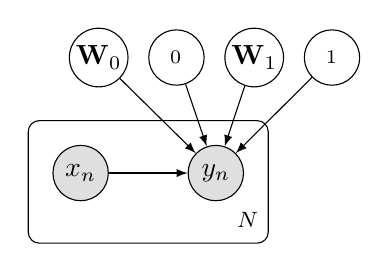
\begin{tikzpicture}

  % Nodes
  \node[latent]              (W0)      {$\mbW_0$} ;
  \node[latent, right=of W0, xshift=-0.75cm]              (b0)      {$\mbb_0$} ;
  \node[latent, right=of b0, xshift=-0.75cm]              (W1)      {$\mbW_1$} ;
  \node[latent, right=of W1, xshift=-0.75cm]              (b1)      {$\mbb_1$} ;
  \node[obs, below=0.75cm of b0, xshift=0.5cm]      (y)    {$y_n$} ;
  \node[obs, left=1.0cm of y] (x)    {$x_n$} ;

  % Edges
  \edge{W0}{y};
  \edge{b0}{y};
  \edge{W1}{y};
  \edge{b1}{y};
  \edge{x}{y};

  % Plates
  \plate[inner sep=0.3cm,
    label={[xshift=-15pt,yshift=15pt]south east:$N$}] {plate1} {
    (y)(x)
  } {};

\end{tikzpicture}

\end{subfigure}%
\\
\begin{subfigure}{\columnwidth}
\begin{lstlisting}[language=python]
W_0 = Normal(loc=tf.zeros([D, H]), sigma=tf.ones([D, H]))
W_1 = Normal(loc=tf.zeros([H, 1]), sigma=tf.ones([H, 1]))
b_0 = Normal(loc=tf.zeros(H), sigma=tf.ones(H))
b_1 = Normal(loc=tf.zeros(1), sigma=tf.ones(1))

x = tf.placeholder(tf.float32, [N, D])
y = Bernoulli(logits=tf.matmul(tf.nn.tanh(tf.matmul(x, W_0) + b_0), W_1) + b_1)
\end{lstlisting}
\end{subfigure}
\caption{}
\end{figure}

\begin{figure}[t]
\begin{subfigure}{0.45\columnwidth}
  \centering
  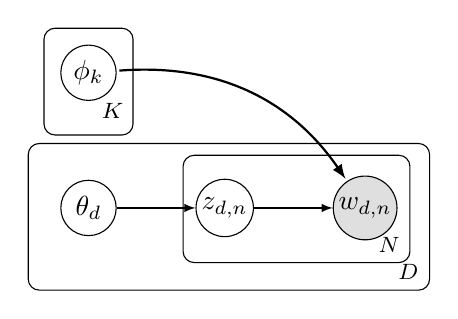
\begin{tikzpicture}

  % Nodes
  \node[latent]               (phi)      {$\phi_k$} ;
  \node[latent, below=1.0cm of phi] (theta)    {$\theta_d$} ;
  \node[latent, right=1.0cm of theta] (z)    {$z_{d,n}$} ;
  \node[obs, right=1.0cm of z]      (w)        {$w_{d,n}$} ;

  % Edges
  \draw[style=arrow, bend left] (phi) to (w);
  \edge{z}{w};
  \edge{theta}{z};

  % Plates
  \plate[inner sep=0.15cm, yshift=0.1cm,
    label={[xshift=-15pt,yshift=13pt]south east:$N$}] {plate1} {
    (w)(z)
  } {};
  \plate[inner sep=0.4cm,
    label={[xshift=-15pt,yshift=13pt]south east:$D$}] {plate2} {
    (w)(z)(theta)
  } {};
  \plate[inner sep=0.2cm,
    label={[xshift=-15pt,yshift=15pt]south east:$K$}] {plate3} {
    (phi)
  } {};

\end{tikzpicture}

\end{subfigure}%
\begin{subfigure}{0.55\columnwidth}
\begin{lstlisting}[language=python]
D = 4  # number of documents
N = [11502, 213, 1523, 1351]  # words per doc
K = 10  # number of topics
V = 100000  # vocabulary size

theta = Dirichlet(alpha=tf.zeros([D, K]) + 0.1)
phi = Dirichlet(alpha=tf.zeros([K, V]) + 0.05)
z = [[0] * N] * D
w = [[0] * N] * D
for d in range(D):
  for n in range(N[d]):
    z[d][n] = Categorical(pi=theta[d, :])
    w[d][n] = Categorical(pi=phi[z[d][n], :])
\end{lstlisting}
\end{subfigure}
\caption{}
\end{figure}

\begin{figure}[t]
\begin{subfigure}{0.35\columnwidth}
  \centering
  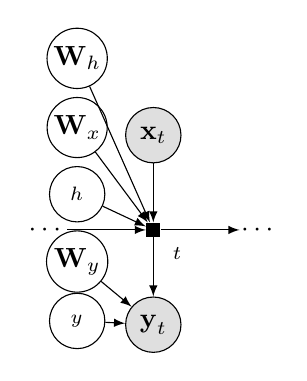
\begin{tikzpicture}

  % Nodes
  \node[empty]              (dot)      {} ;
  \node[obs, right=of dot, xshift=-0.75cm]        (xt) {$\mbx_t$} ;
  \node[latent, left=of xt, xshift=0.75cm, yshift=-0.75cm]  (bh)  {$\mbb_h$} ;
  \node[latent, above=of bh, yshift=-0.9cm]      (Wx) {$\mbW_x$} ;
  \node[latent, above=of Wx, yshift=-0.9cm]      (Wh)      {$\mbW_h$} ;
  \node[latent, below=of bh, yshift=0.9cm]      (Wy)      {$\mbW_y$} ;
  \node[latent, below=of Wy, yshift=1.0cm]      (by)      {$\mbb_y$} ;

  \factor[below=0.75cm of xt] {ht} {} {} {};
  \node[right=0.03cm of ht, yshift=-0.3cm] (htteyt) {$\mbh_t$};
  \node[empty, left=of ht]      (htminus)    {$\cdots$} ;
  \node[empty, right=of ht]      (htplus)    {$\cdots$} ;

  \node[obs, below=0.75cm of ht]      (yt)    {$\mby_t$} ;
  \node[empty, left=of yt]      (ytminus)    {} ;
  \node[empty, right=of yt]      (ytplus)    {} ;

  % Edges
  \edge{Wh}{ht};
  \edge{Wx}{ht};
  \edge{bh}{ht};
  \edge{xt}{ht};
  \edge{Wy}{yt};
  \edge{by}{yt};
  \edge{ht}{yt};
  \edge{htminus}{ht};
  \edge{ht}{htplus};

\end{tikzpicture}

\end{subfigure}%
\begin{subfigure}{0.6\columnwidth}
\begin{lstlisting}[language=python]
def rnn_cell(hprev, xt):
  return tf.tanh(tf.dot(hprev, Wh) + tf.dot(xt, Wx) + bh)

Wh = Normal(loc=tf.zeros([H, H]), scale=tf.ones([H, H]))
Wx = Normal(loc=tf.zeros([D, H]), scale=tf.ones([D, H]))
Wy = Normal(loc=tf.zeros([H, 1]), scale=tf.ones([H, 1]))
bh = Normal(loc=tf.zeros(H), scale=tf.ones(H))
by = Normal(loc=tf.zeros(1), scale=tf.ones(1))

x = tf.placeholder(tf.float32, [None, D])
h = tf.scan(rnn_cell, x, initializer=tf.zeros(H))
y = Normal(loc=tf.matmul(h, Wy) + by, scale=1.0)
\end{lstlisting}
\end{subfigure}
\caption{}
\end{figure}

\begin{figure}[t]
\centering
\begin{lstlisting}[language=Python]
qbeta = PointMass(params=tf.Variable(tf.zeros([K, D])))
qz = Categorical(logits=tf.Variable(tf.zeros([N, K])))

inference_e = ed.VariationalInference({z: qz}, data={x: x_train, beta: qbeta})
inference_m = ed.MAP({beta: qbeta}, data={x: x_train, z: qz})
...
for _ in range(10000):
  inference_e.update()
  inference_m.update()
\end{lstlisting}
\caption{}
\end{figure}

\begin{figure}[t]
\begin{subfigure}{0.35\columnwidth}
  \centering
  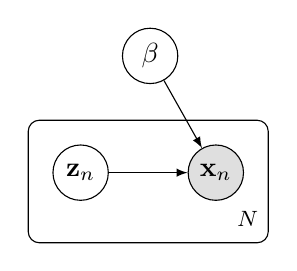
\begin{tikzpicture}

  % Nodes
  \node[latent]               (beta)      {$\beta$} ;
  \node[left=0.4cm of beta]               (betaph)      {} ;
  \node[latent, below=1.0cm of betaph] (z)    {$\mbz_n$} ;
  \node[obs, right=1.0cm of z]      (x)        {$\mbx_n$} ;

  % Edges
  % \edge{beta}{z};
  \edge{beta}{x};
  \edge{z}{x};

  % Plates
  \plate[inner sep=0.3cm,
    label={[xshift=-15pt,yshift=15pt]south east:$N$}] {plate1} {
    (x)(z)
  } {};

\end{tikzpicture}

\end{subfigure}%
\begin{subfigure}{0.6\columnwidth}
  \centering
\begin{lstlisting}[language=python]
N = 10000  # number of data points
D = 2  # data dimension
K = 5  # number of clusters

beta = Normal(loc=tf.zeros([K, D]), scale=tf.ones([K, D]))
z = Categorical(logits=tf.zeros([N, K]))
x = Normal(loc=tf.gather(beta, z), scale=tf.ones([N, D]))
\end{lstlisting}
\end{subfigure}
\caption{}
\end{figure}

\begin{figure}[t]
\begin{subfigure}{0.3\columnwidth}
  \centering
  \input{tikz/hierarchical_model}
\end{subfigure}%
\begin{subfigure}{0.6\columnwidth}
  \centering
\begin{lstlisting}[language=python]
beta = Normal(loc=tf.zeros([K, D]), scale=tf.ones([K, D]))
z = Categorical(logits=tf.zeros([M, K]))
x = Normal(loc=tf.gather(beta, z), scale=tf.ones([M, D]))

qbeta = Normal(loc=tf.Variable(tf.zeros([K, D])),
               scale=tf.nn.softplus(tf.Variable(tf.zeros([K, D]))))
qz = Categorical(logits=tf.Variable(tf.zeros([M, D])))

inference = ed.VariationalInference({beta: qbeta, z: qz}, data={x: x_batch})
inference.initialize(scale={x: float(N)/M, z: float(N)/M})
\end{lstlisting}
\end{subfigure}
\caption{}
\end{figure}

\begin{figure}[t]
\begin{lstlisting}[language=python]
loc = DirichletProcess(0.1, Normal(tf.zeros(D), tf.ones(D)), sample_shape=N)
x = Normal(loc=loc, scale=tf.ones([N, D]))
\end{lstlisting}

\begin{lstlisting}[language=python]
def dirichlet_process(alpha):
  def cond(k, beta_k):
    flip = Bernoulli(p=beta_k)
    return tf.equal(flip, tf.constant(1))

  def body(k, beta_k):
    beta_k = beta_k * Beta(a=1.0, b=alpha)
    return k + 1, beta_k

  k = tf.constant(0)
  beta_k = Beta(a=1.0, b=alpha)
  stick_num, stick_beta = tf.while_loop(cond, body, loop_vars=[k, beta_k])
  return stick_num
\end{lstlisting}
\caption{}
\end{figure}

% \bibliographystyle{iclr2017_conference}
% \bibliography{bib}

\end{document}
